% Created 2021-09-08 mié 11:34
% Intended LaTeX compiler: pdflatex
\documentclass[11pt]{article}
\usepackage[utf8]{inputenc}
\usepackage[T1]{fontenc}
\usepackage{graphicx}
\usepackage{grffile}
\usepackage{longtable}
\usepackage{wrapfig}
\usepackage{rotating}
\usepackage[normalem]{ulem}
\usepackage{amsmath}
\usepackage{textcomp}
\usepackage{amssymb}
\usepackage{capt-of}
\usepackage{hyperref}
\author{Galindo}
\date{\textit{[2021-08-06 vie]}}
\title{Cálculo Multivariable\\\medskip
\large Apuntes}
\hypersetup{
 pdfauthor={Galindo},
 pdftitle={Cálculo Multivariable},
 pdfkeywords={},
 pdfsubject={},
 pdfcreator={Emacs 26.3 (Org mode 9.1.9)}, 
 pdflang={Spanish}}
\begin{document}

\maketitle
\setcounter{tocdepth}{1}
\tableofcontents

\section{Funciones discontinuas más comunes}
\label{sec:org00616e0}
Funciones Discontinuas Más Comunes:
\begin{itemize}
\item Un numero dividido entre 0 es indefinido, por lo tanto una función dividida entre 0 también es indefinida y por lo tanto discontinua.

\item A los números negativos no le podemos sacar raíz cuadrada en el dominio de los números reales.

\item Tangente, en los puntos \(\frac{(2k + 1)\pi}{2}\).

\item Secante, en los puntos \(\frac{(2k + 1)\pi}{2}\).

\item Cosecante, en los puntos \(\pi k\).

\item logaritmo de 10 en \(x \leq 0\)
\end{itemize}

\section{Representación del plano}
\label{sec:orgadf8828}
un plano es un objeto ideal que solo posee dos dimensiones, y contiene infinitos puntos y rectas; es un concepto fundamental de la geometría junto con el punto y la recta. Su ecuación es la siguiente:

\begin{DEMONSTRATION}
\[
ax + by + cz + d = 0
\]
\end{DEMONSTRATION}

otras formas de representar el plano también podrían ser las siguiente:

\section{Ecuación vectorial del plano}
\label{sec:org28f41b9}
\begin{DEMONSTRATION}
\[
\boldsymbol{a} \cdot \boldsymbol{r} = \boldsymbol{n} \cdot \boldsymbol{r}_0
\]
\end{DEMONSTRATION}

\section{Ecuación escalar}
\label{sec:org7c32d6d}
\begin{DEMONSTRATION}
\[
a (x-x_0) + b (y - y_0) + c (z - z_0) = 0
\]
\end{DEMONSTRATION}

\section{Plano Entre Tres Puntos}
\label{sec:org92f5ef7}
Para determinar la funcion que se forma con tres puntos en el espacio, sustituimos los valores y calculamos el determinante de la matriz resultante:

\begin{DEMONSTRATION}
\[ Det \begin{pmatrix}
   x-a_x   & y-a_y   & z-a_z   \\
   b_x-a_x & b_y-a_y & b_z-a_z \\
   c_x-a_x & c_y-a_y & c_x-a_z \\
\end{pmatrix} \]
\end{DEMONSTRATION}

\href{https://github.com/Galindo-lab/calculator/blob/main/eigenmath/plano-entre-3-puntos}{eigenmath} | \href{https://github.com/Galindo-lab/calculator/blob/main/xcas/plano.cas}{KhiCas} 

\section{Ángulo Entre Planos}
\label{sec:orgeda36ae}
para calcular el angulo entre dos planos usamos la siguiente ecuación:

\begin{DEMONSTRATION}
\[
\cos \theta = \frac{\vec{u} \cdot \vec{v}}{\left|\vec{u}\right|\left|\vec{v}\right|}
\]
\end{DEMONSTRATION}

donde n es un punto en \(\mathbb{R}^3\), primero determinamos el valor absoluto de la normal de \(n_1\) y de \(n_2\) y los multiplicamos, ese sera nuestro divisor; Para el denominador calculamos el producto cruz entre \(n_1\) y \(n_2\) y obtenemos su valor de la normal; Y por ultimo calculamos el arco coseno (\(cos^{-1}(\theta)\)) de nuestra división, ojo que el resultado esta en radianes.

\href{https://github.com/Galindo-lab/calculator/blob/main/eigenmath/angulo-entre-dos-planos}{eigenmath} | \href{https://youtu.be/qEVrSjLyOdU}{Video}

\section{Plano que pasa por un punto y es perpendicular a otro plano}
\label{sec:org8339af4}
Para encontrar un plano perpendicular podemos aplicar una de las operaciones de vectores el producto cruz, pero primero tendremos que encontrar el \hyperref[sec:org862a355]{vector de la función}. Y ya con el vector solo tenemos que encontrar el vector perpendicular (producto cruz) y pasamos los valores a la ecuación \hyperref[sec:org7c32d6d]{escalar del plano}:

\begin{DEMONSTRATION}
Punto por el que queremos que pasase la función:
\[
A = (2,3,4)
\]

Función y su forma de vector:
\[ 
3x+2y+z-6=0 \rightarrow B = (3,2,1)
\]

producto cruz (C):
\[
Det \begin{vmatrix}
x & y & z\\
3 & 2 & 1\\
2 & 3 & 4
\end{vmatrix} = (5, -10, 5)
\]

por ultimo sustituimos en la ecuación del plano:
\[
5(x-2)-10(y-3)+5(z-4) = 0
\]

\[
5x-10y+5z = 20+10-30 
\]

\[
\boxed{5x-10y+5z = 0}
\]
\end{DEMONSTRATION}

\href{https://www.youtube.com/watch?v=RkMxfogdWJ0}{Video} 

\section{Vector de una recta o función}
\label{sec:org862a355}
Para obtener el vector de una función simplemente extraemos los valores escalares que están multiplicando a nuestros valores coordenados:

\begin{DEMONSTRATION}
función:
\[ \frac{1}{2} x + 7y - 4z - 6 = 0 \]

su vector:
\[ (\frac{1}{2}, 7, -4) \]
\end{DEMONSTRATION}

\section{Parametrizacion de una recta con dos puntos}
\label{sec:org3af52e6}
Sustituimos los valores en la siguiente formula, P\(_{\text{1}}\) es el punto de origen, P\(_{\text{2}}\) punto final y t es un valor entre 0 y 1

\begin{DEMONSTRATION}
\[
P_1 + t \cdot (P_2 - P_1)
\]
\end{DEMONSTRATION}

\href{../calculadoras/calculo-recta.html}{Calculadora}

\section{Ecuación paramétrica de la recta a una ecuación simétrica}
\label{sec:org667a4ae}
La ecuación simétrica de la recta nos permite encontrar la ecuación continua de la recta\footnote{\[ \frac{x-x_1}{v_1} = \frac{y-y_1}{v_2} \]} simplemente resolviendo la ecuacion en los términos que necesitemos. 

\begin{DEMONSTRATION}
\[
L: \frac{x-x_0}{a_1} = \frac{y-y_0}{a_2} = \frac{z-z_0}{a_3}
\]
\end{DEMONSTRATION}

Para calculara simplemente tenemos que sustituir nuestro punto de paso \(P_0\) y nuestro vector de dirección \(\vec{a}\) en los valores en la formula:

\begin{DEMONSTRATION}
Identificamos nuestro punto de paso y nuestro vector de dirección:

\[
\Bigg\{ \begin{aligned}
     x &= -4 + 2t\\
     y &= -2  \\
     z &= -2 +5t
\end{aligned} 
\]

punto de paso \(P_0 = (-4,-2,-2)\).
vector de dirección \(\vec{a} = (2,0,5)\).

ahora sustituimos:

\[
L: \frac{x-4}{2} = \frac{y-2}{0} = \frac{z-2}{5}
\]

Cuando nos quede 0 en el denominador de alguna ecuación simplemente sustituimos el valor por su igualación a 0:

\[
L: \frac{x-4}{2} = \frac{z-2}{5} \land y = -2
\]
\end{DEMONSTRATION}

\href{https://youtu.be/JMVEYTqdh6c}{Video}


\section{Coordenadas rectangulares, cilíndricas y esféricas}
\label{sec:orgb2f5216}

\begin{OVERFLOW}
\begin{center}
\begin{tabular}{lll}
Rect. & Polares & Esféricas\\
\hline
\(x\) & \(r \cos(\theta)\) & \(\rho \sin(\varphi)\cos(\theta)\)\\
\(y\) & \(r \sin(\theta)\) & \(\rho \sin(\varphi)\sin(\theta)\)\\
\(z\) & \(z\) & \(\rho \cos(\varphi)\)\\
\(x^2+y^2\) & \(r^2\) & \\
\(x^2+y^2+z^2\) &  & \(\rho^2\)\\
\(y/x\) & \(\tan(\theta)\) & \(\tan(\theta)\)\\
 & \(r\) & \(\rho \sin(\varphi)\)\\
 & \(\theta\) & \(\theta\)\\
\end{tabular}
\end{center}
\end{OVERFLOW}

\section{Coordenadas rectangulares a esfericas}
\label{sec:orgd28ba87}
Las coordenadas esféricas requieren dos ángulos, por lo que se parecen mucho a las coordenadas polares. \(\theta\) funciona exactamente como en coordenadas polares, sí \(x=0\) y \(y > 0\) el ángulo es 90°; sí \(x=0\) y \(y < 0\) el ángulo es 270°.

\begin{DEMONSTRATION}
\[ \begin{aligned} 
r &= \sqrt{x^2+y^2+z^2} & \varphi &= cos^{-1}\left( \frac{z}{r} \right) \\
\end{aligned} 
\]

\[\theta = tan^{-1}\left( \frac{y}{x} \right)\]
\end{DEMONSTRATION}
\href{http://www.learningaboutelectronics.com/Articulos/Calculadora-de-conversion-de-coordenadas-cartesianas-a-esfericas.php\#respuesta}{Calculadora}


\section{Dominio de una función}
\label{sec:org8660baa}
\begin{quote}
Los valores para los cuales la función está definida. Variable independiente
\end{quote}

El dominio son los valores de X que puede tomar una función:

\begin{DEMONSTRATION}
\[ f \begin{pmatrix} x \\ y \end{pmatrix} \ = \frac{ \sqrt{x+y+1} }{x - 1} \]
\end{DEMONSTRATION}

La primera cosa que debemos tomar en cuenta en que puntos la función es discontinua, en este caso la función tiene dos discontinuidades, en el numerador y en el denominador. 

En el denominador no puede haber un número cero, entonces solo basta con resolver la ecuación \(x-1 = 0\) para encontrar la discontinuidad. \(x = 1\)

Como los números negativos no tienen raíces, no hay números reales que multiplicados sean negativos, se puede inferir que la función no existe en ningún punto que donde \(x+y+1 < 0\).

Entonces, con la información que ya conocemos podemos decir que la función existe en todos los puntos donde \(x+y+1\) sea mayor a 0 y donde X sea diferente de 0. En notación matemática el dominio se escribiría así:

\begin{DEMONSTRATION}
\[ \begin{Bmatrix}
  \begin{pmatrix} 
  x \\ y \\ 
  \end{pmatrix} \in \mathbb R^2: 
  x + y + 1 \geq 0 \wedge x \not = 1
\end{Bmatrix}  \]
\end{DEMONSTRATION}

\href{https://youtu.be/qDr0R7hIjts}{Video}

\section{Imagen de una función (Rango)}
\label{sec:orgc29eaf4}
\begin{quote}
Conjunto de valores que puede tomar la función.
Variable dependiente.
\end{quote}

El rango o imagen de una función es todo valor de Y que puede tomar nuestra función \(f: \mathbb R^n \to \mathbb R^m\):

\begin{itemize}
\item Sí la función a la cual queremos calcular su rango solo tiene un parámetro, significa que nos encontramos con una función vectorial \(n = 1\).

\item Por otro lado sí la función acepta dos parámetros y retorna un tercero entonces estamos ante una superficie. \(n = 2\) y \(m = 3\).
\end{itemize}

\begin{DEMONSTRATION}
\[ f \begin{pmatrix} x \\ y \end{pmatrix} = \sqrt{9-x^2-y^2} \]
\end{DEMONSTRATION}

Para encontrar el rango es muy recomendable encontrar primero el \hyperref[sec:org8660baa]{dominio} de la función, así podemos saber donde debemos empezar a evaluar, para nuestro ejemplo el dominio de la función es \({ (^x_y) \in \mathbb R^2: x^2 + y^2 \leq 9 }\).

La primera cosa que podemos notar en la función es que es una raíz, eso significa que no puede ser un valor negativo, por lo tanto el valor mas pequeño al que podemos calcular la raíz en el dominio de los reales es el número 0, este sería el valor mínimo de la imagen.

También podemos notar que los valores están elevados al cuadrado (los valores de X\(^{\text{2}}\) y y\(^{\text{2}}\) siempre son positivos) entonces sus valores siempre se le restan a 9 y entonces como siempre se van a restar los valores, podemos inferir que el valor más alto que puede retornar esta función es \(\sqrt{9}\), este sería el valor máximo de la imagen. 

El resultado que obtenemos es que el dominio de la función se extiende continuamente desde \([0, 3]\).

\href{https://youtu.be/qDr0R7hIjts}{Video}

\section{Curvas de nivel}
\label{sec:orgf6fb0b6}

\begin{center}
\begin{center}
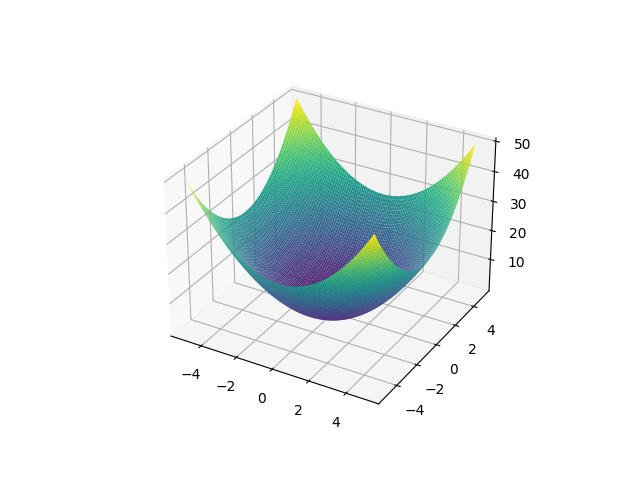
\includegraphics[width=7cm]{./img/test.png}
\end{center}

\begin{center}
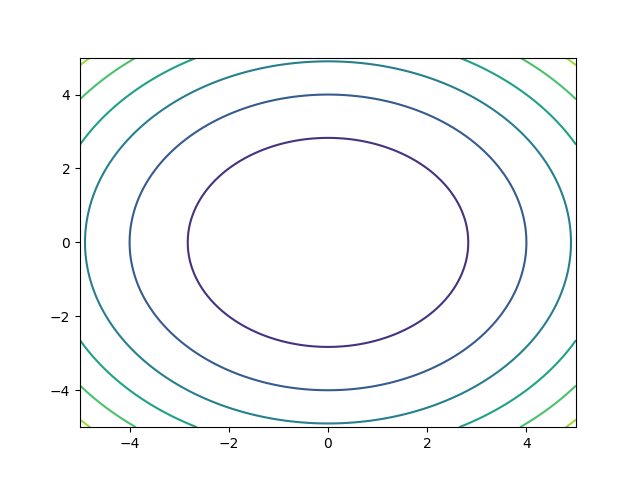
\includegraphics[width=7cm]{./img/test2.png}
\end{center}
\end{center}
\end{document}
